\section{Univariate analysis}
\label{sec:univariate}

\subsection{Raw data}

In my data one chess game forms one data point. Lichess API allows me to extract following information regarding one game: string describing the event (for example whether it was casual or rated game i.e. affected players rating \cite{elo} or no), URL to the game, date and time when game occurred, usernames of both players, ELO rating of both players, result of the game, rating change of both players after the game, game variant and time control, reason for game result which in addition winning by mate can be a problem with internet connection, ECO code \cite{eco} of the opening and all moves in the game using algebraic notation \cite{notation}. In addition to these possible titles of the player such as International Master or Grand Master are given and well as two additional fields regarding Chess 960 variant games. Following provides an example of the API output:

\begin{lstlisting}[breaklines]
    [Event "Rated Rapid game"]
    [Site "https://lichess.org/oykful3u"]
    [Date "2020.06.19"]
    [White "martoj13"]
    [Black "aitotumainen"]
    [Result "1-0"]
    [UTCDate "2020.06.19"]
    [UTCTime "06:12:07"]
    [WhiteElo "1920"]
    [BlackElo "1919"]
    [WhiteRatingDiff "+6"]
    [BlackRatingDiff "-6"]
    [Variant "Standard"]
    [TimeControl "600+0"]
    [ECO "B01"]
    [Termination "Normal"]
    1. e4 d5 2. e5 Nc6 3. Bb5 a6 4. Bxc6+ bxc6 5. d4 Bf5 6. Nd2 e6 7. c3 c5 8. Ne2 cxd4 9. Qa4+ Qd7 10. Qxd7+ Kxd7 11. cxd4 Bd3 12. Nf4 Bb5 13. a3 c5 14. dxc5 Bxc5 15. Nb3 Bf8 16. Nd4 Ne7 17. Be3 Nf5 18. Nxf5 exf5 19. Nxd5 Re8 20. f4 Bc6 21. Rd1 Bxd5 22. Rxd5+ Kc6 23. Rd2 f6 24. Bd4 g5 25. g3 h5 26. Kf2 h4 27. Rc1+ Kb7 28. Rcc2 hxg3+ 29. hxg3 Rh2+ 30. Kg1 Rh3 31. Kg2 Rh7 32. exf6 gxf4 33. gxf4 Bh6 34. Rf2 Re4 35. Be5 Bf8 36. Rf3 Kb6 37. Rg3 Bc5 38. Rg7 Rh4 39. f7 Re1 40. Rxc5 1-0
\end{lstlisting}

In following analysis I study only relations between Result, UTCDate, UTCTime, WhiteElo, BlackElo, Variant and TimeControl. By common sense text strings such as username and event description shouldn't affect the game result. Rating differences are calculated after the game has ended so they can't be explaining factors for the result of the game. I also discard game opening and move information. While this information is definitely meaningful analyzing it would be very complex as already after two moves standard chess game can be in 400 different states and tree of possible game continuations grows unmanageable. For those who are interested on how opening affects game's outcome Lichess Opening Explorer \cite{opening_explorer} and Lichess Game Insights \cite{insights} offer tools for such analysis.

\subsection{Summary statistics from my games}

In total I have played 9085 chess games between 15.02.2016 - 25.03.2021 on this site. Table \ref{tbl:results by variant} shows how games are distributed between different variants \cite{variants} and how game results are distributed inside variant. I have made distinction inside standard chess between games with at least 10 minutes and games with less than 10 minutes on the clock as amount of available time changes nature of the game significantly. In proceeding analysis I will only focus on standard and crazyhouse variants as they have the greatest number of games.

\begin{table}[ht]
    \centering
    \label{tbl:results by variant}
    \caption{Results by chess variant.}
    \begin{tabular}{lllll}
    Chess variant    & wins & draws & losses & win rate\\
    \hline
    Atomic& 138& 7& 120& 0.52 \\
    Crazyhouse& 1732& 15& 2535& 0.40 \\
    Standard short time control& 1162& 70& 1581& 0.41 \\
    From Position& 5& 0& 5& 0.5 \\
    Standard long time control& 794& 79& 712& 0.50 \\
    King of the Hill& 34& 0& 33& 0.51 \\
    Chess960& 9& 1& 12& 0.41 \\
    Three-check& 6& 0& 9& 0.4 \\
    Racing Kings& 8& 0& 8& 0.5 \\
    Horde& 1& 0& 7& 0.13 \\
    Antichess& 2& 0& 0& 1.0
    \end{tabular}
\end{table}


\subsection{Exploratory visualizations of the game data}

Figure \ref{fig:games vs time of day} shows who many games I have played at each hour of day and how many of them I have won and lost and their difference. Image shows that on short standard games and crazyhouse games I am losing more often than winning and on the other hand playing long standard games I win more often. This is consistent with figures in table \ref{tbl:results by variant}. One interesting observation is that between 2 and 3 PM I seem to perform unusually well when playing long standard chess as I win two thirds of my matches. Similarly I win half my crazyhouse games while on other hours of day I am losing more often. Only reason I think of causing this is my habit to drink cup of coffee around that time of day which probably gives me a cognitive boost. 


\begin{figure}[ht!]
    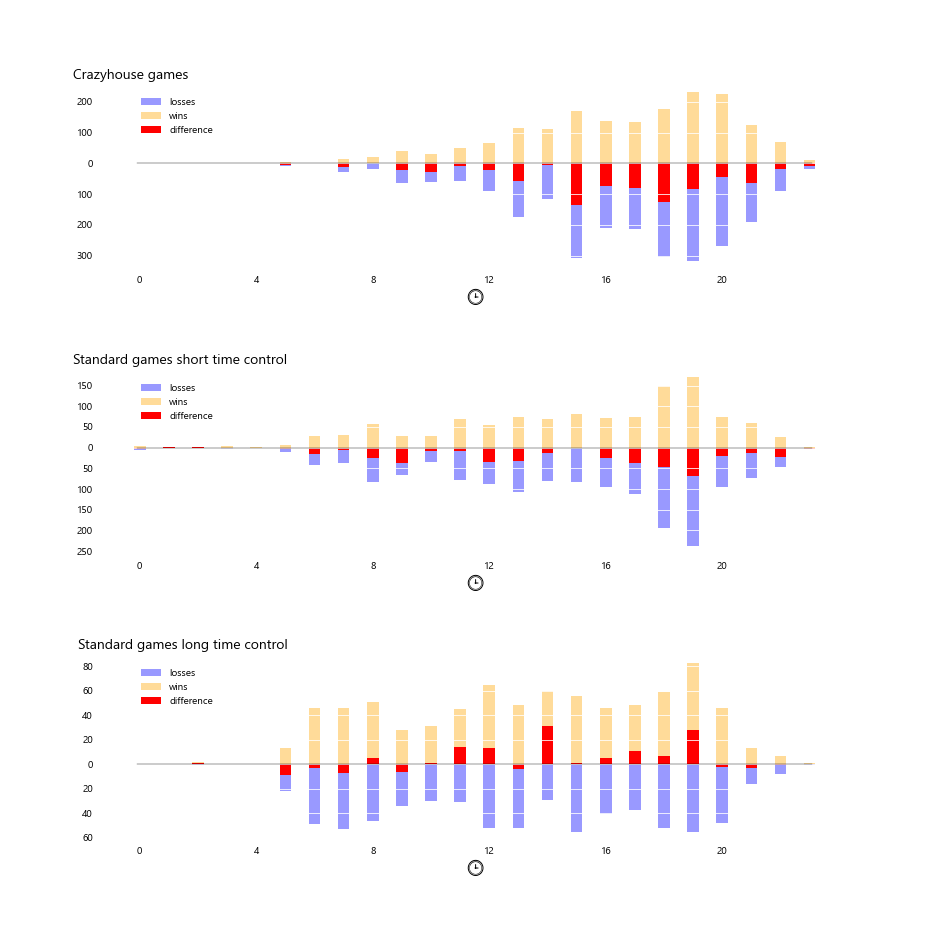
\includegraphics[width=\textwidth]{../img/games_vs_time_of_day.png}
    \caption{Wins and losses with respect to the time of the day.}
    \label{fig:games vs time of day}
\end{figure}

Figure \ref{fig:winning probabilities} shows histogram where rating difference of me and my opponent is divided to 20 equally wide bins and winning probability inside each bin is calculated. In standard chess (both long and short) winning probability seems to decrease in remarkably linear fashion with respect to increasing opponent strength. On the other hand crazyhouse variant has long tails: I have won opponents that are over 800 rating points better than me and vice versa also lost to opponent that are much weaker than me. It must be noted in this image middle bins contain much more data than bins on edges and also selected number of bins affects to the appearance of the graph.

\begin{figure}[ht!]
    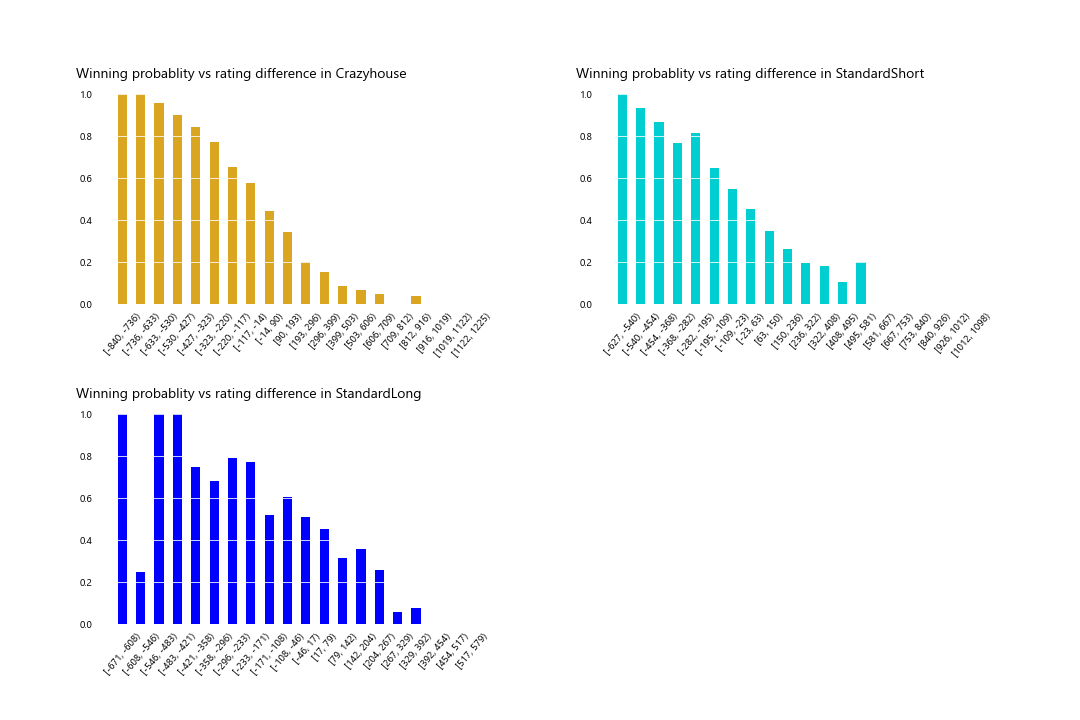
\includegraphics[width=\textwidth]{../img/winning_probabilities_vs_rating.png}
    \caption{Histogram showing winning probability in each bin when rating difference between me and opponent is divided to equally wide bins.}
    \label{fig:winning probabilities}
\end{figure}